Les seules simulations que nous avons pu faire dans le cadre du stage sont des tests pour vérifier la stabilité de nos conditions initiales, ce qui représente déjà un travail important.

Nous avons donc commencé par générer des amas comportant un faible nombre de particules (~1000 ou 5000 particules~) afin de vérifier notre générateur, ce sont les résultats montrés par la courbe~\ref{Comp_gene-theo} pour 5000 particules, puis~\ref{potentiel_5000} pour 100000 particules.
Il nous faut maintenant vérifier que ces amas restent stables sur un grand nombre de temps dynamiques. Les simulations présentées dans cette section utilisent un amas réel dont les données ont été récupéré dans le catalogue de
\textsc{Harris} et à partir du travail fait dans les chapitres précédents. Il s'agit de l'amas NGC 288. Pour cet amas, les calculs analytiques donnent $\alpha = 439.72$.

Passons maintenant à l'étude de la stabilité sur le "long" terme de nos amas. Nous montrerons ici les résultats des tests
décrits dans la section~\ref{Verif_gene}.

Dans la table~\ref{eps_Neps}, nous avons indiqué quelles valeurs de $\epsilon$ nous avons utilisées : la valeur de $N_\epsilon$ correspondante, le nombre de particules qui sont au-delà du rayon des conditions initiales de l'objet,
et quelques autres informations utiles pour trouver la valeur qui nous intéresse.
	\begin{table}[h!]
		\begin{center}
			\begin{tabular}{|c|c|c|c|c|c|}
				\hline
				\multirow{2}{1cm}{$\epsilon\ \(pc\)$}	&	\multirow{2}{1cm}{$N_\epsilon$}	&	\multirow{2}{1cm}{$N_\mathrm{out}$}	&	\multirow{2}{3.5cm}{Fraction d'énergie cinétique emportée}	&	\multirow{2}{3.5cm}{Fraction d'énergie potentielle emportée}	&	\multirow{2}{2cm}{Courbes associées} \\
					&	&	&	&	&	\\
				\hline
				\hline
				$0.0194028$	&	$ 0.44 $		&	380	&	$ 0.00013573$			&	$ 0.00081092$	&	\ref{soft::0.019}, \ref{soft::0.019-Ax}\\
				\hline
				$0.05$		&	$ 7.52 $		&	239	&	$ 8.04628\times 10^{-5}$	&	$ 0.000488421$	&	\ref{soft::0.05}, \ref{soft::0.05-Ax}\\
				\hline
				$0.15$		&	$ 203.17 $		&	282	&	$ 9.91201\times 10^{-5}$	&	$ 0.00106241$	&	\ref{soft::0.15}, \ref{soft::0.15-Ax}\\
				\hline
				$0.20$		&	$ 481.58 $		&	653	&	$ 0.000265688$			&	$ 0.00265207$	&	\ref{soft::0.2}, \ref{soft::0.2-Ax}\\
				\hline
				$0.30$		&	$ 1625.34 $		&	919	&	$ 0.000433181$			&	$ 0.00466071$	&	\ref{soft::0.3}, \ref{soft::0.3-Ax}\\
				\hline
			\end{tabular}
		\end{center}
		\caption{Valeurs testés pour $\epsilon$ et $N_\epsilon$\label{eps_Neps}}
	\end{table}

	Discutons maintenant les résultats.

	\begin{description}
	%\paragraph{$\epsilon = 0.0194028$ :}
	\item[$\epsilon = 0.0194028$]
	Ce paramètre donne des résultats satisfaisants : sa densité évolue assez peu sur le temps de la simulation comparé aux valeur de $\epsilon > 0.05$, et ses axes d'inertie restent constant
	(~le bruit visible sur les graphes est dû au bruit statistique, bruit statistique dû au nombre fini de particules~). Par contre, le nombre de particules dans un volume de taille $\epsilon$ est trop petit : nous sommes trop loin de la limite fluide.

	%\paragraph{$\epsilon = 0.05$ :}
	\item[$\epsilon = 0.05$]
	Les fractions d'énergie potentielle et cinétique emportées par les particules sortantes sont minimum pour ce paramètre. De plus, sa densité et ses axes d'inertie évoluent peu, comme pour la valeur précédente.
	Cette fois, nous avons suffisamment de particules dans le volume de taille $\epsilon$.

\begin{figure}[h!]
	\centering 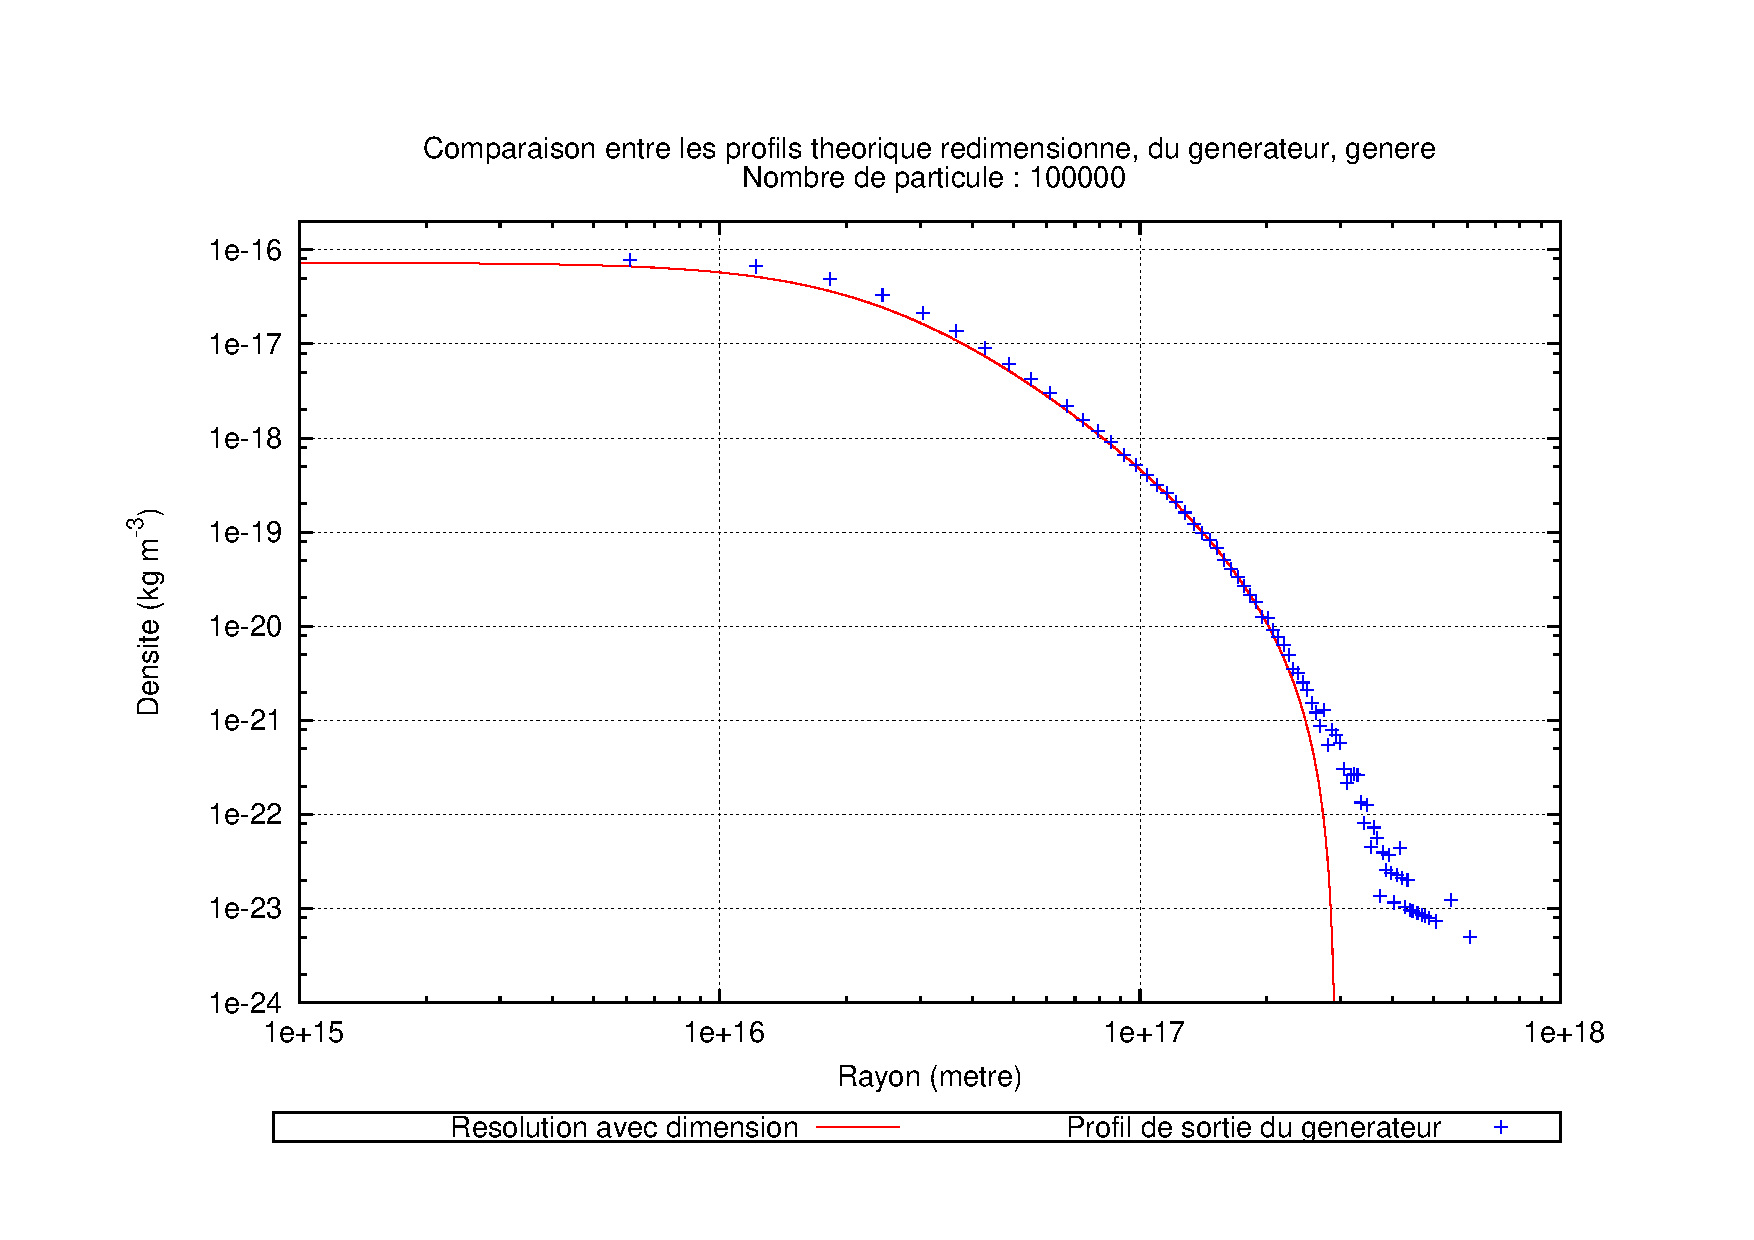
\includegraphics[scale=0.5]{graphe/Comp_dens_gene-theo_0-05.pdf}
	\caption{Comparaison entre la densité numérique et la densité après évolution : $\epsilon = 0.05$\label{soft::0.05}}
\end{figure}

\begin{figure}[h!]
	\centering 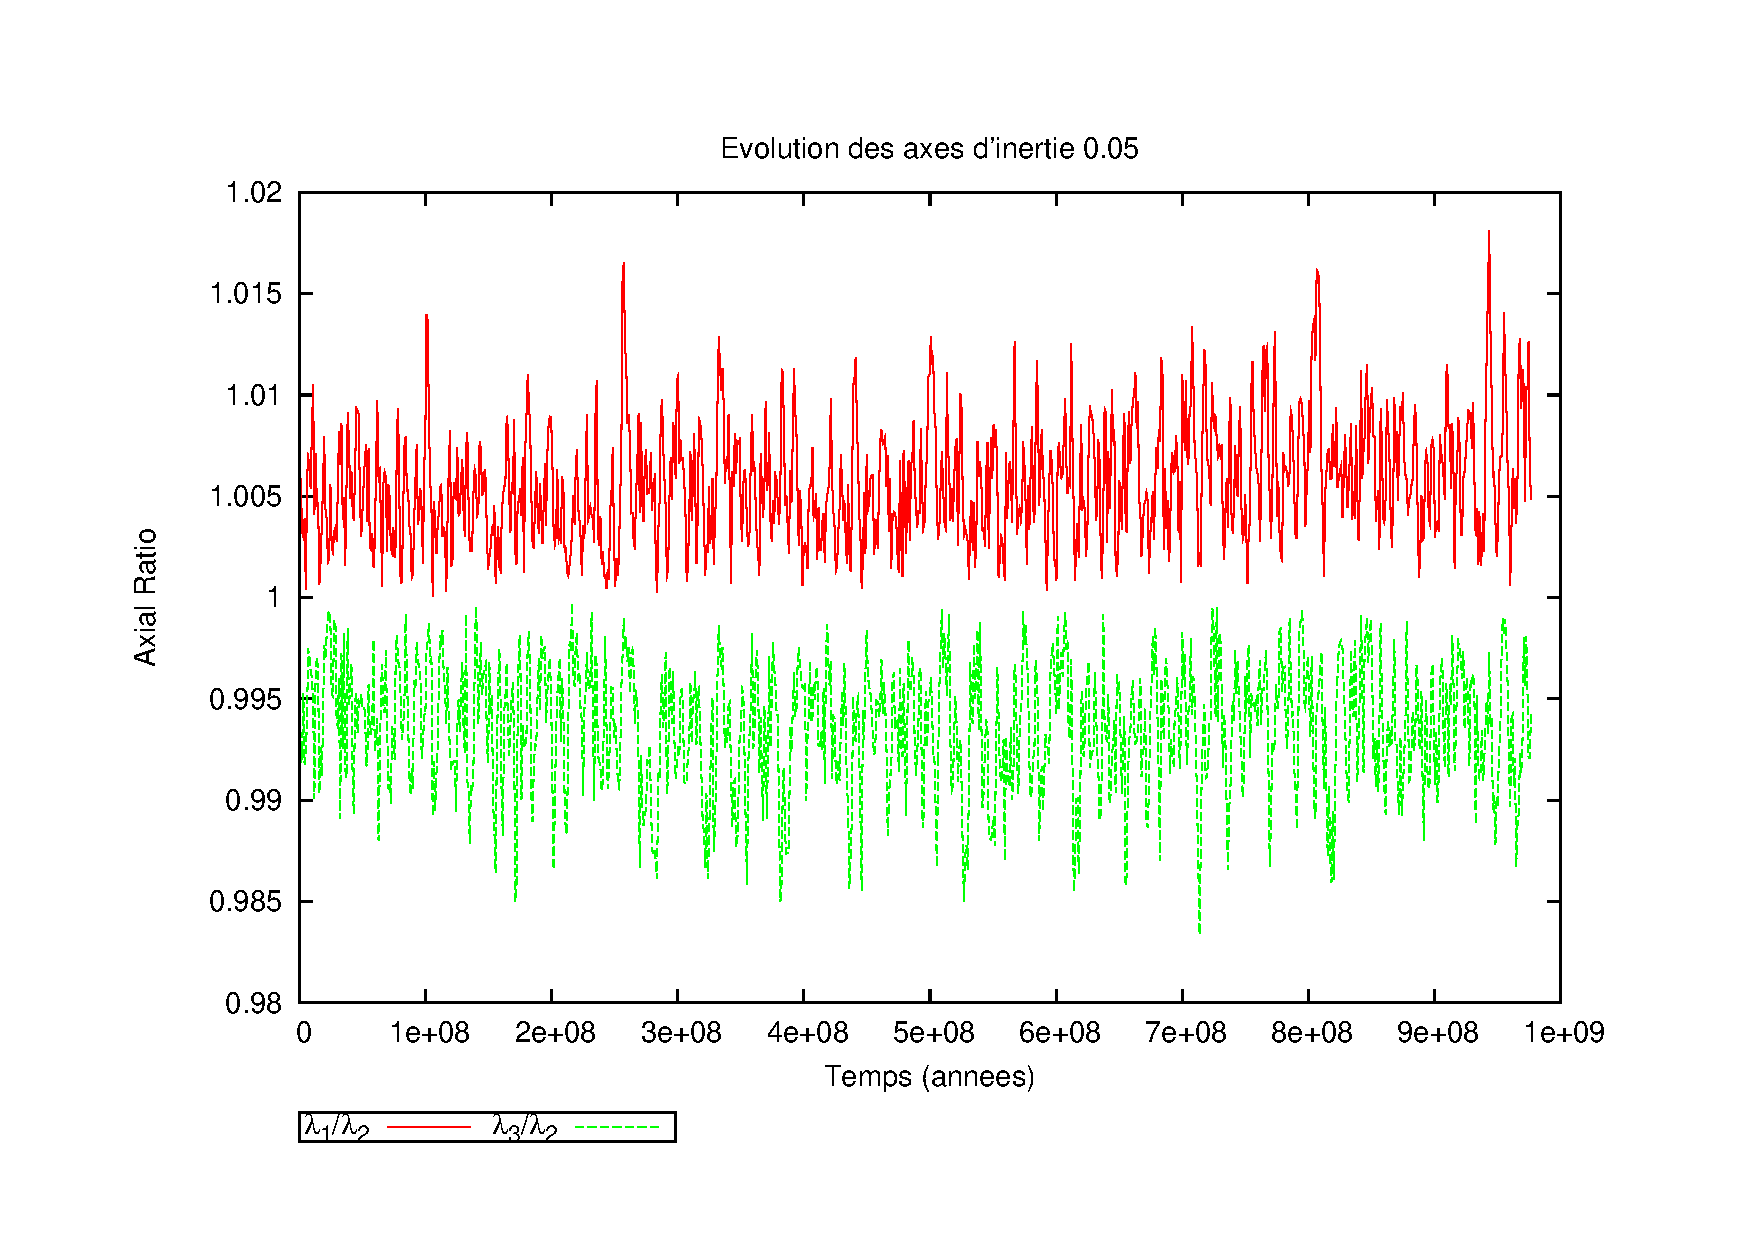
\includegraphics[scale=0.5]{graphe/Axial_ratio_0-05.pdf}
	\caption{Évolution des rapports des axes d'inertie : $\epsilon = 0.05$\label{soft::0.05-Ax}}
\end{figure}

	%\paragraph{$\epsilon = 0.15$ :}
	\item[$\epsilon = 0.15$]
	Pour ce paramètre, la fraction d'énergie potentielle emportée est de l'ordre de $0.1\%$, ce qui représente un changement important pour le rapport du Viriel $2 E_c/E_p$
	(~avec $E_c$ l'énergie cinétique et $E_p$ l'énergie potentielle~) : le profil de densité a complétement changé, l'amas s'est étendu.
	Par contre, il commence à se passer des choses intéressantes au niveau des axes d'inertie : pendant une grande partie de la simulation l'amas conserve sa forme, puis une instabilité arrive et il se déforme. % selon
%	l'un des axes, mais reste constant sur le second.
	\item[$\epsilon > 0.15$]
	Les valeurs supérieurs de $\epsilon$ ne sont alors clairement pas intéressante. De plus, ces valeurs sont trop proches du rayon de cœur de l'amas qui est de l'ordre de $10^{16}\ m = 0.32\ pc$ : en lissant toute
	la partie centrale de l'amas, nous changeons sa dynamique. En effet, il suffit de voir que, en augmentant le paramètre de lissage, l'instabilité menant à une déformation arrive de plus en plus tôt.
	Les déformations deviennent plus violentes.
	\end{description}

	La valeur de lissage optimale se trouve donc entre $\epsilon = 0.05$ et $\epsilon = 0.15$, pour une dizaine de particule (~pour $N_\epsilon = 10$, $\epsilon \sim 0.05497\ pc$~).

